\documentclass{ximeraXloud}
\usepackage{longdivision}
\usepackage{polynom}
\usepackage{float}% Use `H' as the figure optional argument to force it's vertical placement to conform to source.
%\usepackage{caption}% Allows us to describe the figures without having "figure 1:" in it. :: Apparently Caption isn't supported.
%    \captionsetup{labelformat=empty}% Actually does the figure configuration stated above.
\usetikzlibrary{arrows.meta,arrows}% Allow nicer arrow heads for tikz.
\usepackage{gensymb, pgfplots}
\usepackage{tabularx}
\usepackage{arydshln}



\graphicspath{
  {./}
  {./explorePolynomials/}
  {./exploreRadicals/}
  {./graphing/}
}

%% Default style for tikZ
\pgfplotsset{my style/.append style={axis x line=middle, axis y line=
middle, xlabel={$x$}, ylabel={$y$}, axis equal }}


%% Because log being natural log is too hard for people.
\let\logOld\log% Keep the old \log definition, just in case we need it.
\renewcommand{\log}{\ln}


%%% Changes in polynom to show the zero coefficient terms
\makeatletter
\def\pld@CF@loop#1+{%
    \ifx\relax#1\else
        \begingroup
          \pld@AccuSetX11%
          \def\pld@frac{{}{}}\let\pld@symbols\@empty\let\pld@vars\@empty
          \pld@false
          #1%
          \let\pld@temp\@empty
          \pld@AccuIfOne{}{\pld@AccuGet\pld@temp
                            \edef\pld@temp{\noexpand\pld@R\pld@temp}}%
           \pld@if \pld@Extend\pld@temp{\expandafter\pld@F\pld@frac}\fi
           \expandafter\pld@CF@loop@\pld@symbols\relax\@empty
           \expandafter\pld@CF@loop@\pld@vars\relax\@empty
           \ifx\@empty\pld@temp
               \def\pld@temp{\pld@R11}%
           \fi
          \global\let\@gtempa\pld@temp
        \endgroup
        \ifx\@empty\@gtempa\else
            \pld@ExtendPoly\pld@tempoly\@gtempa
        \fi
        \expandafter\pld@CF@loop
    \fi}
\def\pld@CMAddToTempoly{%
    \pld@AccuGet\pld@temp\edef\pld@temp{\noexpand\pld@R\pld@temp}%
    \pld@CondenseMonomials\pld@false\pld@symbols
    \ifx\pld@symbols\@empty \else
        \pld@ExtendPoly\pld@temp\pld@symbols
    \fi
    \ifx\pld@temp\@empty \else
        \pld@if
            \expandafter\pld@IfSum\expandafter{\pld@temp}%
                {\expandafter\def\expandafter\pld@temp\expandafter
                    {\expandafter\pld@F\expandafter{\pld@temp}{}}}%
                {}%
        \fi
        \pld@ExtendPoly\pld@tempoly\pld@temp
        \pld@Extend\pld@tempoly{\pld@monom}%
    \fi}
\makeatother




%%%%% Code for making prime factor trees for numbers, taken from user Qrrbrbirlbel at: https://tex.stackexchange.com/questions/131689/how-to-automatically-draw-tree-diagram-of-prime-factorization-with-latex

\usepackage{forest,mathtools,siunitx}
\makeatletter
\def\ifNum#1{\ifnum#1\relax
  \expandafter\pgfutil@firstoftwo\else
  \expandafter\pgfutil@secondoftwo\fi}
\forestset{
  num content/.style={
    delay={
      content/.expanded={\noexpand\num{\forestoption{content}}}}},
  pt@prime/.style={draw, circle},
  pt@start/.style={},
  pt@normal/.style={},
  start primeTree/.style={%
    /utils/exec=%
      % \pt@start holds the current minimum factor, we'll start with 2
      \def\pt@start{2}%
      % \pt@result will hold the to-be-typeset factorization, we'll start with
      % \pgfutil@gobble since we don't want a initial \times
      \let\pt@result\pgfutil@gobble
      % \pt@start@cnt holds the number of ^factors for the current factor
      \def\pt@start@cnt{0}%
      % \pt@lStart will later hold "l"ast factor used
      \let\pt@lStart\pgfutil@empty,
    alias=pt-start,
    pt@start/.try,
    delay={content/.expanded={$\noexpand\num{\forestove{content}}
                            \noexpand\mathrlap{{}= \noexpand\pt@result}$}},
    primeTree},
  primeTree/.code=%
    % take the content of the node and save it in the count
    \c@pgf@counta\forestove{content}\relax
    % if it's 2 we're already finished with the factorization
    \ifNum{\c@pgf@counta=2}{%
      % add the factor
      \pt@addfactor{2}%
      % finalize the factorization of the result
      \pt@addfactor{}%
      % and set the style to the prime style
      \forestset{pt@prime/.try}%
    }{%
      % this simply calculates content/2 and saves it in \pt@end
      % this is later used for an early break of the recursion since no factor
      % can be greater then content/2 (for integers of course)
      \edef\pt@content{\the\c@pgf@counta}%
      \divide\c@pgf@counta2\relax
      \advance\c@pgf@counta1\relax % to be on the safe side
      \edef\pt@end{\the\c@pgf@counta}%
      \pt@do}}

%%% our main "function"
\def\pt@do{%
  % let's test if the current factor is already greather then the max factor
  \ifNum{\pt@end<\pt@start}{%
    % great, we're finished, the same as above
    \expandafter\pt@addfactor\expandafter{\pt@content}%
    \pt@addfactor{}%
    \def\pt@next{\forestset{pt@prime/.try}}%
  }{%
    % this calculates int(content/factor)*factor
    % if factor is a factor of content (without remainder), the result will
    % equal content. The int(content/factor) is saved in \pgf@temp.
    \c@pgf@counta\pt@content\relax
    \divide\c@pgf@counta\pt@start\relax
    \edef\pgf@temp{\the\c@pgf@counta}%
    \multiply\c@pgf@counta\pt@start\relax
    \ifNum{\the\c@pgf@counta=\pt@content}{%
      % yeah, we found a factor, add it to the result and ...
      \expandafter\pt@addfactor\expandafter{\pt@start}%
      % ... add the factor as the first child with style pt@prime
      % and the result of int(content/factor) as another child.
      \edef\pt@next{\noexpand\forestset{%
        append={[\pt@start, pt@prime/.try]},
        append={[\pgf@temp, pt@normal/.try]},
        % forest is complex, this makes sure that for the second child, the
        % primeTree style is not executed too early (there must be a better way).
        delay={
          for descendants={
            delay={if n'=1{primeTree, num content}{}}}}}}%
    }{%
      % Alright this is not a factor, let's get the next factor
      \ifNum{\pt@start=2}{%
        % if the previous factor was 2, the next one will be 3
        \def\pt@start{3}%
      }{%
        % hmm, the previos factor was not 2,
        % let's add 2, maybe we'll hit the next prime number
        % and maybe a factor
        \c@pgf@counta\pt@start
        \advance\c@pgf@counta2\relax
        \edef\pt@start{\the\c@pgf@counta}%
      }%
      % let's do that again
      \let\pt@next\pt@do
    }%
  }%
  \pt@next
}

%%% this builds the \pt@result macro with the factors
\def\pt@addfactor#1{%
  \def\pgf@tempa{#1}%
  % is it the same factor as the previous one
  \ifx\pgf@tempa\pt@lStart
    % add 1 to the counter
    \c@pgf@counta\pt@start@cnt\relax
    \advance\c@pgf@counta1\relax
    \edef\pt@start@cnt{\the\c@pgf@counta}%
  \else
    % a new factor! Add the previous one to the product of factors
    \ifx\pt@lStart\pgfutil@empty\else
      % as long as there actually is one, the \ifnum makes sure we do not add ^1
      \edef\pgf@tempa{\noexpand\num{\pt@lStart}\ifnum\pt@start@cnt>1 
                                           ^{\noexpand\num{\pt@start@cnt}}\fi}%
      \expandafter\pt@addfactor@\expandafter{\pgf@tempa}%
    \fi
    % setup the macros for the next round
    \def\pt@lStart{#1}% <- current (new) factor
    \def\pt@start@cnt{1}% <- first time
  \fi
}
%%% This simply appends "\times #1" to \pt@result, with etoolbox this would be
%%% \appto\pt@result{\times#1}
\def\pt@addfactor@#1{%
  \expandafter\def\expandafter\pt@result\expandafter{\pt@result \times #1}}

%%% Our main macro:
%%% #1 = possible optional argument for forest (can be tikz too)
%%% #2 = the number to factorize
\newcommand*{\PrimeTree}[2][]{%
  \begin{forest}%
    % as the result is set via \mathrlap it doesn't update the bounding box
    % let's fix this:
    tikz={execute at end scope={\pgfmathparse{width("${}=\pt@result$")}%
                         \path ([xshift=\pgfmathresult pt]pt-start.east);}},
    % other optional arguments
    #1
    % And go!
    [#2, start primeTree]
  \end{forest}}
\makeatother


\providecommand\tabitem{\makebox[1em][r]{\textbullet~}}
\providecommand{\letterPlus}{\makebox[0pt][l]{$+$}}
\providecommand{\letterMinus}{\makebox[0pt][l]{$-$}}



\title{Polynomial Long Division}
\begin{document}
\begin{abstract}
    Factor out a polynomial using long division
\end{abstract}
\maketitle

Many of the sections remaining in this topic are methods to find \textit{roots} or \textit{zeros} of a polynomial, but not how to \textit{factor} the polynomial. You may wonder how it is that it's a section on `factoring' if it specifically \textit{doesn't} factor the polynomial. That's where the `Polynomial Division' part comes in. This is why, before we get to those sections, we pause to learn these division tools. Although not directly factoring related, polynomial division allows one to factor a polynomial if you already know a root (or zero) of the polynomial.%
\footnote{%
    This may seem like a weirdly specific situation, but in truth it happens surprisingly often, especially once we have the rational root theorem. Moreover, these techniques of division, and especially the `polynomial long division' can be generalized into other techniques in higher level math classes.%
    }%

\subsection{Polynomial Long Division}
    The most general (and arguably useful) version of polynomial division is the \textit{polynomial long division}. The key idea to learn and remember this technique is that it is \textit{exactly} the same process as you \textit{first} learned to do regular long division with numbers. It has probably been a little while since you last used long division in its most formal way though, so we will give a quick rehash here. This may seem silly, but it is \textit{extremely} helpful when it comes to learning polynomial long division, so don't skip this part thinking that you already know how to do long division, trust me on this!
    
    \begin{image}
        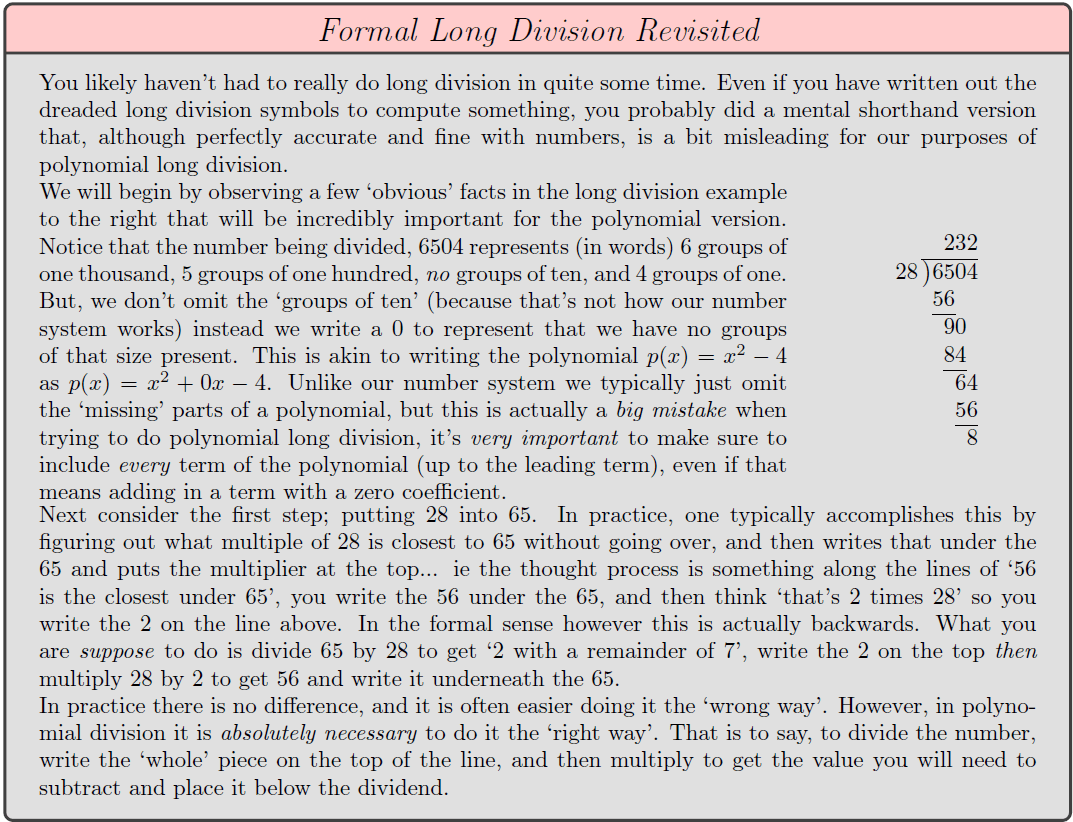
\includegraphics[width=\textwidth]{formalLongDivisionRevisited.png}
    \end{image}%
    
    
    %\begin{explanation}
    %    Formal Long Division Revisited%
    %    
    %    You likely haven't had to really do long division in quite some time. Even if you have written out the dreaded long division symbols to compute something, you probably did a mental shorthand version that, although perfectly accurate and fine with numbers, is a bit misleading for our purposes of polynomial long division.
    %
    %    \begin{minipage}[t]{0.75\linewidth}
    %        We will begin by observing a few `obvious' facts in the long division example to the right that will be incredibly important for the polynomial version. Notice that the number being divided, $6504$ represents (in words) $6$ groups of one thousand, $5$ groups of one hundred, \textit{no} groups of ten, and $4$ groups of one. But, we don't omit the `groups of ten' (because that's not how our number system works) instead we write a $0$ to represent that we have no groups of that size present. This is akin to writing the polynomial $p(x) = x^2 - 4$ as $p(x) = x^2 + 0x - 4$. Unlike our number system we typically just omit the `missing' parts of a polynomial, but this is actually a \textit{big mistake} when trying to do polynomial long division, it's \textit{very important} to make sure to include \textit{every} term of the polynomial (up to the leading term), even if that means adding in a term with a zero coefficient.
    %    \end{minipage}
    %    \begin{minipage}[t]{0.2\linewidth}
    %        \vspace*{0.5cm}
    %        \begin{center}
    %            \intlongdivision{6504}{28}
    %        \end{center}
    %    \end{minipage}
    %    Next consider the first step; putting $28$ into $65$. In practice, one typically accomplishes this by figuring out what multiple of $28$ is closest to $65$ without going over, and then writes that under the $65$ and puts the multiplier at the top... ie the thought process is something along the lines of `$56$ is the closest under $65$', you write the $56$ under the $65$, and then think `that's $2$ times $28$' so you write the $2$ on the line above. In the formal sense however this is actually backwards. What you are \textit{suppose} to do is divide $65$ by $28$ to get `$2$ with a remainder of $7$', write the $2$ on the top \textit{then} multiply $28$ by $2$ to get $56$ and write it underneath the $65$.
    %
    %    In practice there is no difference, and it is often easier doing it the `wrong way'. However, in polynomial division it is \textit{absolutely necessary} to do it the `right way'. That is to say, to divide the number, write the `whole' piece on the top of the line, and then multiply to get the value you will need to subtract and place it below the dividend.
    %\end{explanation}% End Formal Long Division Rehash
    
    \subsection*{Ok, I am having some kind of PTSD flashbacks to elementary school now, thanks for that...}
        Yea, I know, this seems silly. But polynomial long division works \textit{exactly} like the \textit{\textbf{formal}} version of long division. Unfortunately, the \textit{formal} version of long division isn't really the version that people use and think about. As a result, people often try to do polynomial long division using their own mental short-cut version of long division... which works great for numbers, and goes horribly horribly awry with polynomials. Hopefully the formal long division revisited above will help clarify the subtle differences between how you probably remember long division, and how it's \textit{technically} suppose to be done (even if nobody actually does it that way).
    
    \subsection*{Fair enough, I forgot some of that, but can we do the polynomial division now?}
        I'll take that tone to be one of eager enthusiasm, because I'm sure it wasn't the weary hostility it sounded like.
        
        Polynomial division follows the exact same process as the formal long division above. Specifically we want to write out the divisor (thing we are dividing by) and dividend (the thing we are dividing) in the same spots and then go through the steps outlined above.
    
        \begin{image}
            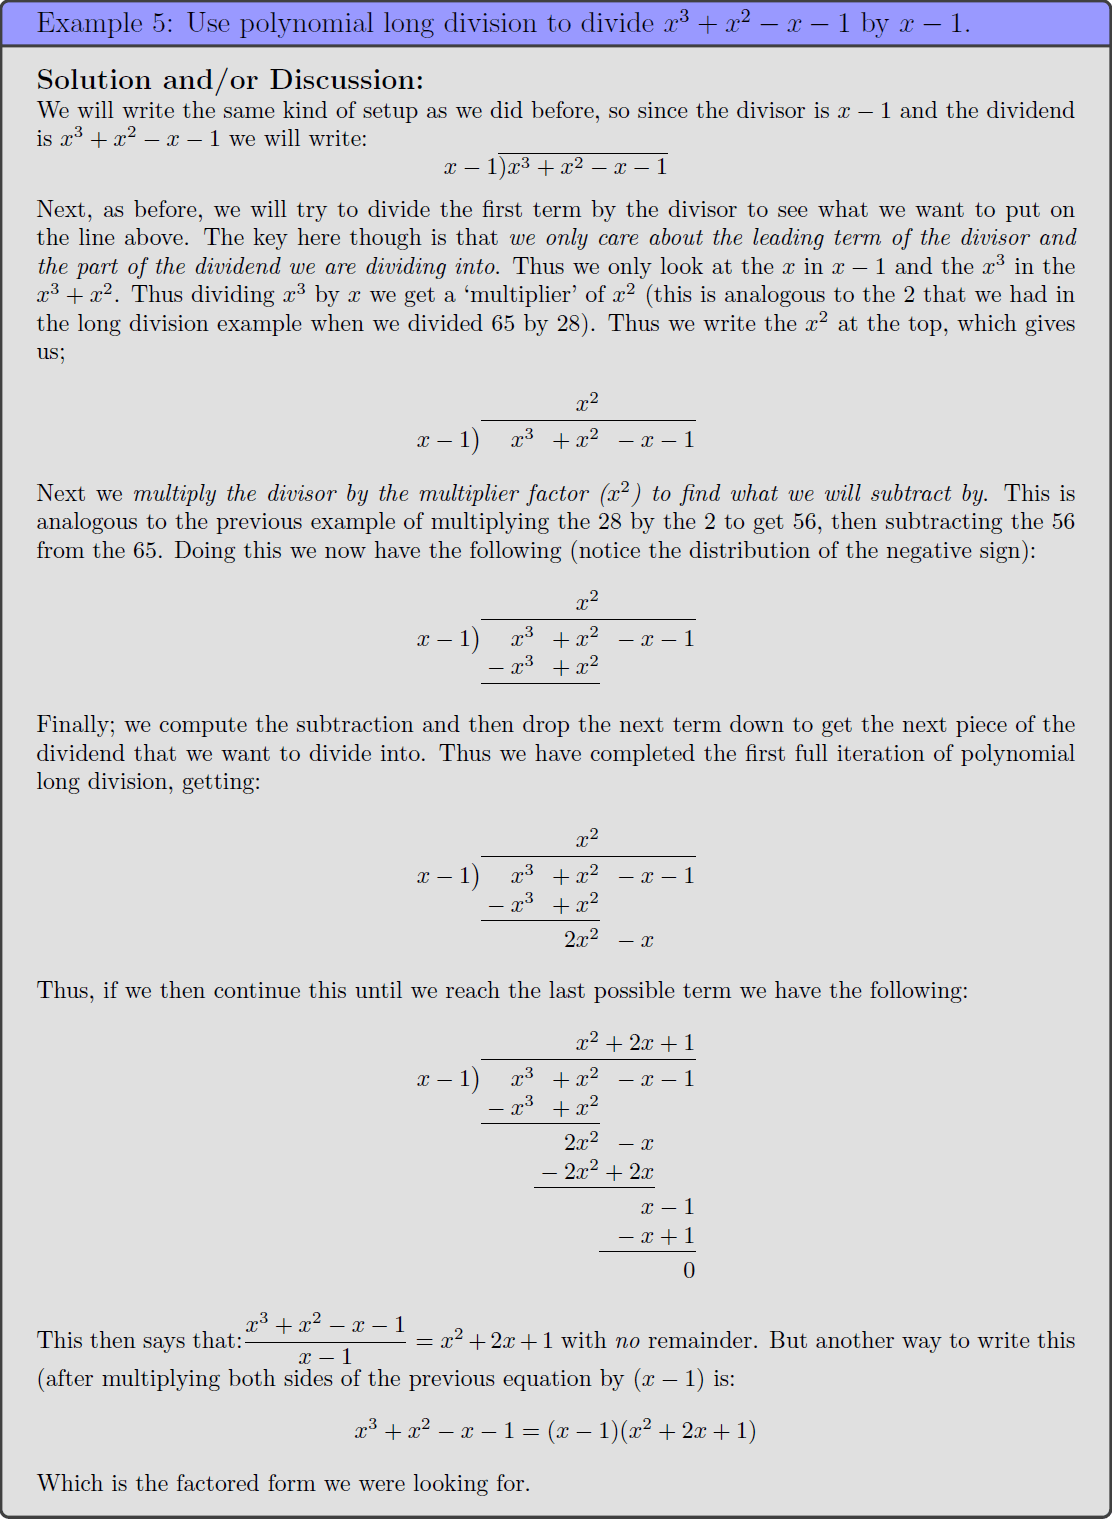
\includegraphics[width=\textwidth]{exPolyLongDivision.png}
        \end{image}
        
        
    %\begin{example}
    %    Use polynomial long division to divide $x^3 + x^2 - x - 1$ by $x - 1$.\\%
    %    
    %    We will write the same kind of setup as we did before, so since the divisor is $x - 1$ and the dividend is $x^3 + x^2 - x - 1$ we will write:
    %    \[
    %        x - 1 \overline{)x^3 + x^2 - x - 1}
    %    \]
    %    Next, as before, we will try to divide the first term by the divisor to see what we want to put on the line above. The key here though is that \textit{we only care about the leading term of the divisor and the part of the dividend we are dividing into}. Thus we only look at the $x$ in $x - 1$ and the $x^3$ in the $x^3 + x^2$. Thus dividing $x^3$ by $x$ we get a `multiplier' of $x^2$ (this is analogous to the $2$ that we had in the long division example when we divided 65 by 28). Thus we write the $x^2$ at the top, which gives us;
    %
    %    \begin{center}
    %        \polylongdiv[stage=2]{x^3 + x^2 - x - 1}{x - 1}
    %    \end{center}
    %
    %    Next we \textit{multiply the divisor by the multiplier factor ($x^2$) to find what we will subtract by}. This is analogous to the previous example of multiplying the 28 by the 2 to get 56, then subtracting the 56 from the 65. Doing  this we now have the following (notice the distribution of the negative sign):
    %
    %    \begin{center}
    %        \polylongdiv[stage=3]{x^3 + x^2 - x - 1}{x - 1}
    %    \end{center}
    %
    %    Finally; we compute the subtraction and then drop the next term down to get the next piece of the dividend that we want to divide into. Thus we have completed the first full iteration of polynomial long division, getting:
    %
    %    \begin{center}
    %        \polylongdiv[stage=4]{x^3 + x^2 - x - 1}{x - 1}
    %    \end{center}
    %
    %    Thus, if we then continue this until we reach the last possible term we have the following:
    %
    %    \begin{center}
    %        \polylongdiv{x^3 + x^2 - x - 1}{x - 1}
    %    \end{center}
    %
    %    This then says that:$ \dfrac{x^3 + x^2 - x - 1}{x - 1} = x^2 + 2x + 1$ with \textit{no} remainder. But another way to write this (after multiplying both sides of the previous equation by ($x-1$) is:
    %    \[
    %        x^3 + x^2 - x  - 1 = (x - 1)(x^2 + 2x + 1)
    %    \]
    %    Which is the factored form we were looking for.
    %\end{example}%.
    
    
    \subsection*{Ok, but what happens when we have a non-zero remainder?}
    
        Great question! The short answer is, you realize you've chosen poorly... the thing you hoped was a root, was not. That isn't to say the polynomial long division failed. Indeed, let's look at the example above but divide by $x-2$ instead of $x-1$. Then we get:
        
        \begin{image}
            
\includegraphics[width=\textwidth]{exPolyLongDivisionTwo.png}
        \end{image}
        
        %\begin{center}
        %    \polylongdiv{x^3 + x^2 - x - 1}{x - 2}
        %\end{center}
        
        Now, just like with doing regular long division, if you have a remainder you have some choices. With numeric long division, if you were to divide, say, 45 by 7, you'd get 6 with a remainder of 3. You could proceed to find a decimal version, but sevenths tend to suck. Instead we could write it as $\frac{45}{7} = 6 + \frac{3}{7}$. This is exactly what we do with polynomials. Using the above polynomial long division we have a remainder of 9, the way we would write the result would be:
        \[
            x^3 + x^2 - x - 1 = (x - 2)\left(x^2 + 3x + 5 + \dfrac{9}{x-2}\right)
        \]
        This is perfectly correct, but as we can see one of the `factors' is no longer a polynomial... and once that happens a lot of our tools vanish. Thus, although technically correct, it's not actually useful.
    


\end{document}